\documentclass[MSc]{podunipdthesis}
\usepackage{lipsum}
\usepackage[Lenny]{fncychap}

\begin{document}

\author{Albert Einstein}
\title{The equation of everything}
\aayear{2020/2021}

\begin{supervisors}
   \supervisor{Chiar.mo}{Prof.}{A. Nyone}
   \supervisor{}{Dr.}{S. One Else}
\end{supervisors}

\begin{cosupervisors}
   \cosupervisor{Chiar.ma}{Prof.ssa}{E. Noether}
   \cosupervisor{}{Dr.}{S. Kovalevskaya}
\end{cosupervisors}

%\phdname{physics} % default
%\phdname{science of materials}
%\phdname{complex systems}

\maketitlepage

\tableofcontents

\chapter*{Introduction}
\addcontentsline{toc}{chapter}{Introduction}

\lipsum[20]

\chapter{State of the art}

\section{Section title}

\subsection{Subsection title}

\lipsum[20] \cite{Resnick:03} \lipsum[5]

\lipsum[40]
Inline equation $\nabla\cdot{\bf B} = 0$.
\lipsum[20]

\begin{figure}[t]
\centering
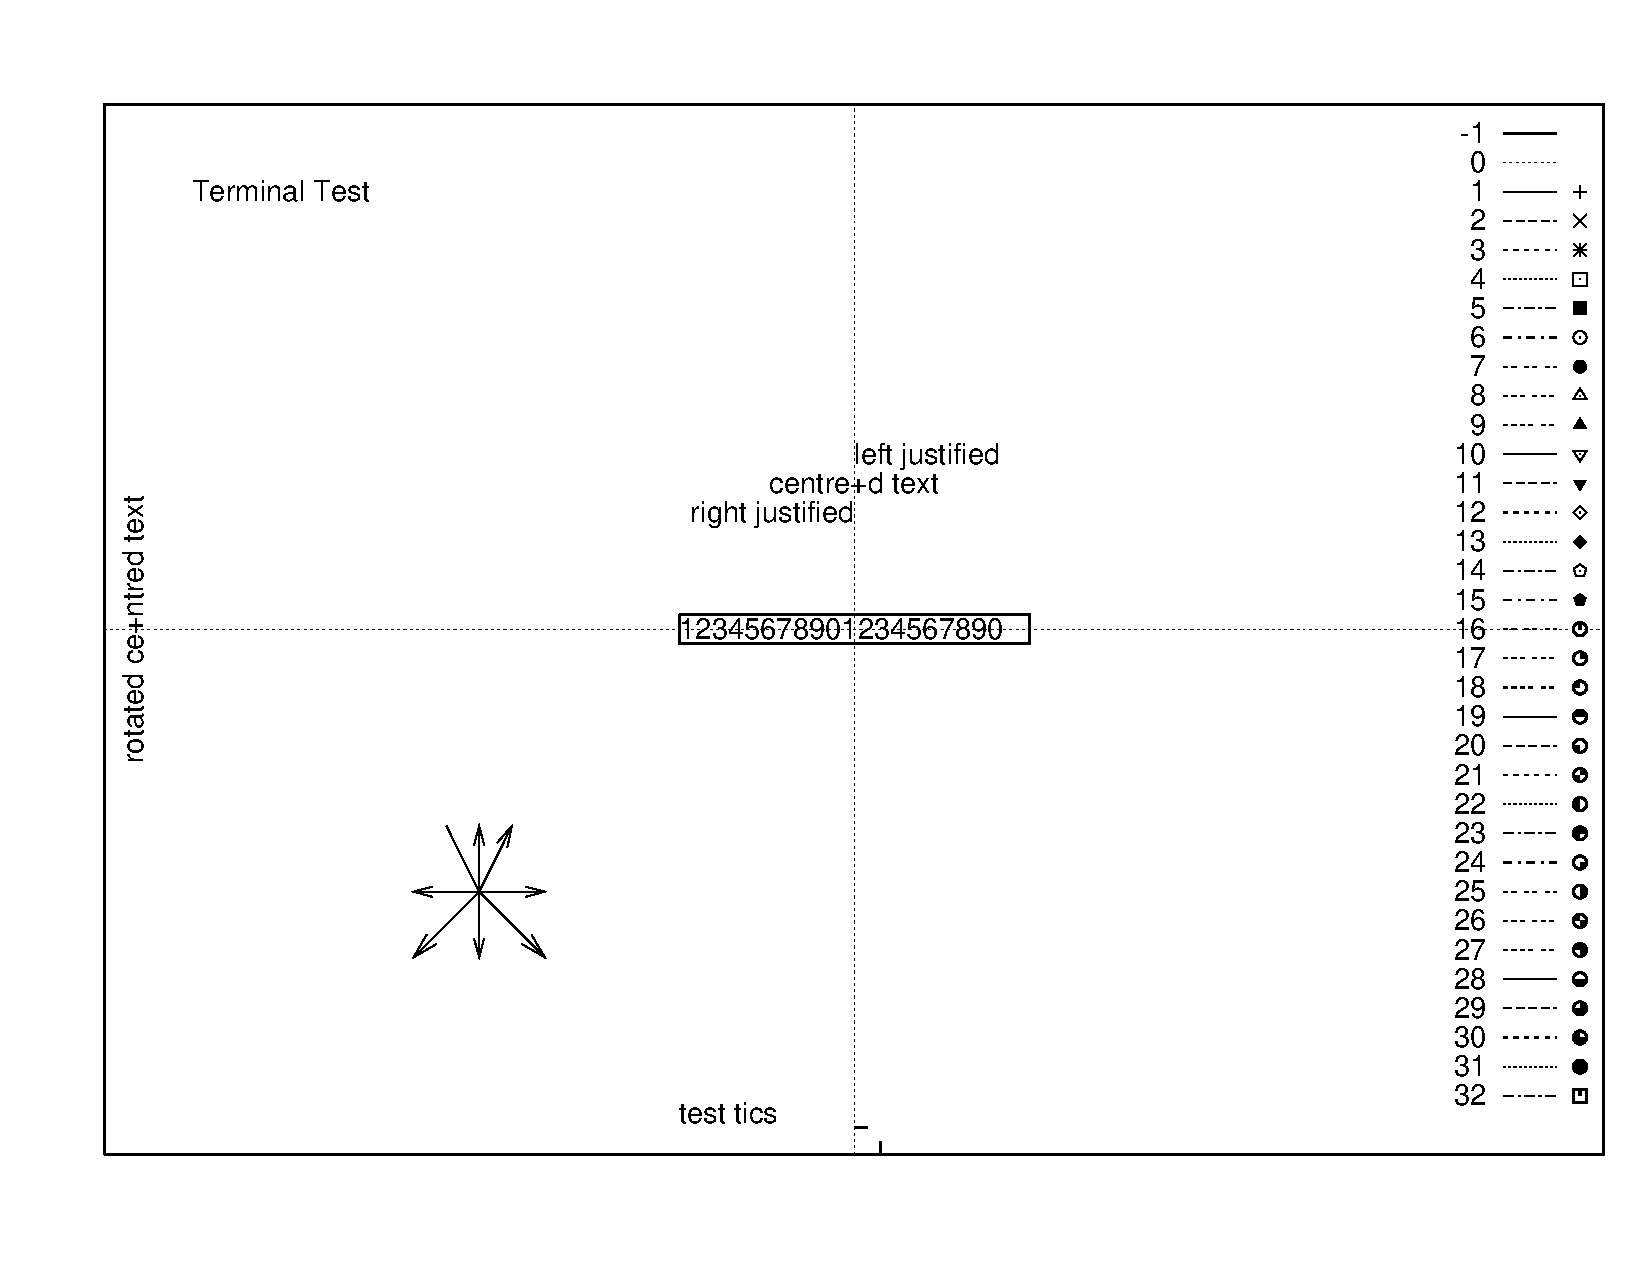
\includegraphics[width=0.8\columnwidth]{esempio.pdf}
\caption{Caption}
\label{fig:esempio}
\end{figure}

Cf.\ Fig.~\ref{fig:esempio}.
\lipsum[30]
\begin{equation}
f(z) = \oint \frac{f(\zeta)}{\zeta - z} d\zeta .
\end{equation}
\lipsum[10]

\chapter*{Conclusions}
\addcontentsline{toc}{chapter}{Conclusions}

\lipsum[20]

\addcontentsline{toc}{chapter}{Bibliography}
\bibliographystyle{mprsty}
\bibliography{biblio}

\chapter*{Acknowledgements}
\addcontentsline{toc}{chapter}{Acknowledgements}

\lipsum[20]

\end{document}
